\documentclass[tikz,border=7pt]{standalone}
\usepackage[T1]{fontenc}
\usepackage{lmodern}
\usepackage{helvet}
\renewcommand{\familydefault}{\sfdefault}
\usepackage{amsmath}
\usepackage{xcolor}
\usepackage{tikz}
\usetikzlibrary{
  arrows.meta,
  positioning,
  calc,
  fit,
  shapes.geometric,
  shapes.symbols,
  backgrounds,
  decorations.pathreplacing,
  decorations.pathmorphing,
}

\definecolor{slate}{HTML}{334155}
\definecolor{teal}{HTML}{0D9488}
\definecolor{amber}{HTML}{D97706}
\definecolor{rose}{HTML}{E11D48}
\definecolor{muted}{HTML}{64748B}
\definecolor{line}{HTML}{94A3B8}
\definecolor{pagebg}{HTML}{F8FAFC}
\definecolor{card}{HTML}{FFFFFF}
\definecolor{lightteal}{HTML}{CCFBF1}
\definecolor{lightamber}{HTML}{FEF3C7}
\definecolor{lightrose}{HTML}{FFE4E6}
\definecolor{lightslate}{HTML}{E2E8F0}
\definecolor{blueink}{HTML}{2563EB}
\definecolor{bluewash}{HTML}{DBEAFE}
\definecolor{greenink}{HTML}{16A34A}
\definecolor{greenwash}{HTML}{DCFCE7}
\definecolor{pinkink}{HTML}{DB2777}
\definecolor{pinkwash}{HTML}{FCE7F3}

\tikzset{
  >=Stealth,
  font=\sffamily\scriptsize,
  every node/.append style={text=slate},
  title/.style={font=\sffamily\bfseries\small, text=slate, anchor=west},
  note/.style={font=\sffamily\tiny, text=muted, align=left},
  label/.style={font=\sffamily\tiny, text=muted},
  chip/.style={
    draw=#1,
    fill=#1!12,
    rounded corners=2pt,
    inner sep=2.5pt,
    font=\sffamily\tiny\bfseries,
    text=slate,
  },
  decision/.style={
    shape=diamond,
    aspect=2.1,
    draw=teal,
    fill=lightteal,
    inner sep=1.5pt,
    align=center,
    font=\sffamily\tiny,
    text=slate,
  },
  pics/person/.style 2 args={
    code={
      \fill[#1] (0,0.92) circle (0.18);
      \fill[#1]
        (-0.26,0.68)
        .. controls (-0.34,0.42) and (-0.30,0.18) .. (-0.22,0.02)
        -- (0.22,0.02)
        .. controls (0.30,0.18) and (0.34,0.42) .. (0.26,0.68)
        -- cycle;
      \node[font=\sffamily\tiny\bfseries, text=#1, anchor=north] at (0,-0.08) {#2};
    }
  },
  pics/disk/.style={
    code={
      \fill[lightslate] (0,-0.04) ellipse (0.28 and 0.10);
      \fill[slate] (-0.28,-0.04) rectangle (0.28,0.12);
      \fill[slate] (0,0.12) ellipse (0.28 and 0.10);
      \fill[card] (0,0.14) ellipse (0.11 and 0.04);
    }
  },
}

\begin{document}
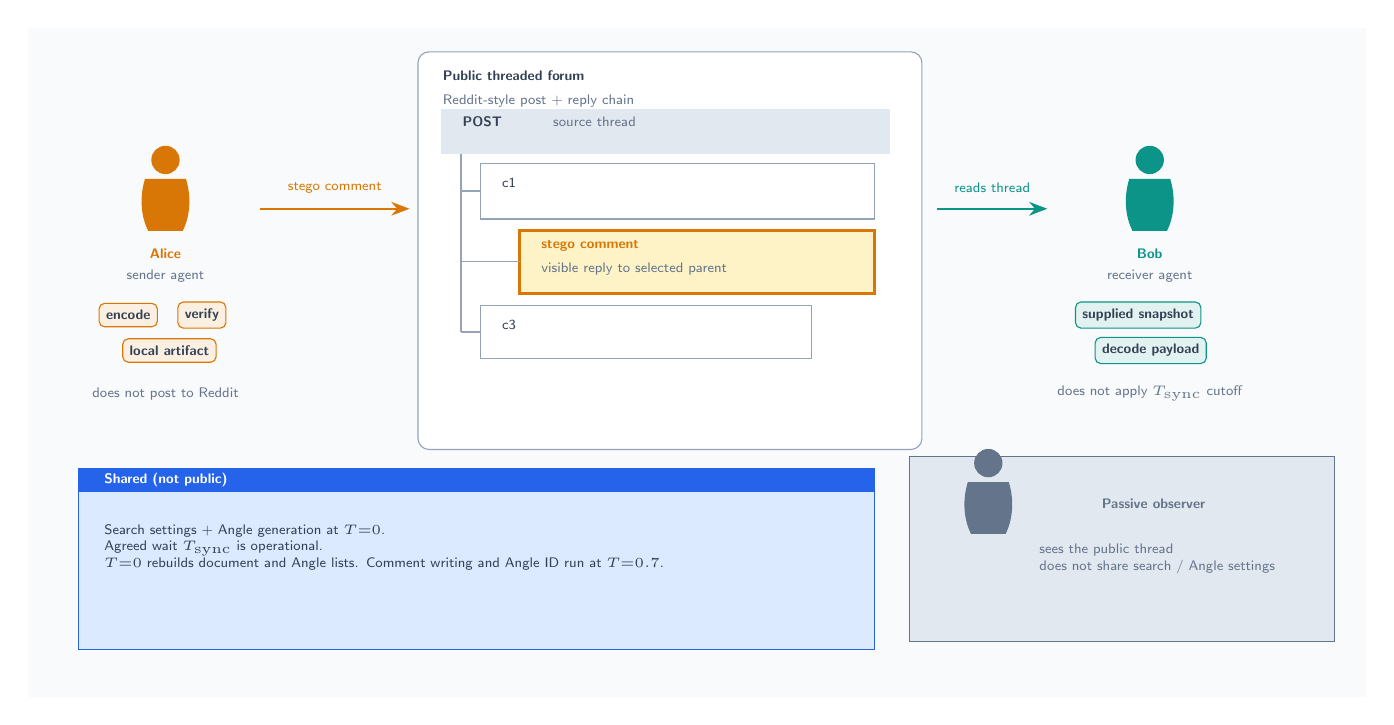
\begin{tikzpicture}[x=1cm,y=1cm]
  \fill[pagebg] (-0.4,-0.35) rectangle (16.6,8.15);

  % Alice
  \begin{scope}[shift={(1.35,5.55)}]
    \pic {person={amber}{Alice}};
    \node[font=\sffamily\tiny, text=muted, align=center] at (0,-0.55) {sender agent};
    \node[chip=amber, anchor=west] at (-0.85,-1.05) {encode};
    \node[chip=amber, anchor=west] at (0.15,-1.05) {verify};
    \node[chip=amber, anchor=west] at (-0.55,-1.50) {local artifact};
    \node[note, align=center, text width=3.1cm] at (0,-2.05) {does not post to Reddit};
  \end{scope}

  % Thread mock
  \node[
    draw=line, fill=card, rounded corners=4pt,
    minimum width=6.4cm, minimum height=5.05cm, anchor=north west,
  ] (forum) at (4.55,7.85) {};
  \node[font=\sffamily\tiny\bfseries, text=slate, anchor=north west] at (4.75,7.72) {Public threaded forum};
  \node[label, anchor=north west] at (4.75,7.42) {Reddit-style post + reply chain};

  \fill[lightslate] (4.85,6.55) rectangle (10.55,7.12);
  \node[font=\sffamily\tiny\bfseries, anchor=west] at (5.0,6.95) {POST};
  \node[label, anchor=west] at (6.15,6.95) {source thread};

  \fill[card] (5.35,5.72) rectangle (10.35,6.42);
  \draw[line] (5.35,5.72) rectangle (10.35,6.42);
  \node[font=\sffamily\tiny, anchor=west] at (5.5,6.18) {c1};
  \fill[lightamber] (5.85,4.78) rectangle (10.35,5.58);
  \draw[amber, line width=1.1pt] (5.85,4.78) rectangle (10.35,5.58);
  \node[font=\sffamily\tiny\bfseries, text=amber, anchor=west] at (6.0,5.38) {stego comment};
  \node[label, anchor=west] at (6.0,5.08) {visible reply to selected parent};
  \fill[card] (5.35,3.95) rectangle (9.55,4.62);
  \draw[line] (5.35,3.95) rectangle (9.55,4.62);
  \node[font=\sffamily\tiny, anchor=west] at (5.5,4.38) {c3};
  \draw[line, line width=0.7pt] (5.10,6.55) -- (5.10,4.28);
  \draw[line, line width=0.7pt] (5.10,6.07) -- (5.35,6.07);
  \draw[line, line width=0.7pt] (5.10,5.18) -- (5.85,5.18);
  \draw[line, line width=0.7pt] (5.10,4.28) -- (5.35,4.28);

  % Bob
  \begin{scope}[shift={(13.85,5.55)}]
    \pic {person={teal}{Bob}};
    \node[font=\sffamily\tiny, text=muted, align=center] at (0,-0.55) {receiver agent};
    \node[chip=teal, anchor=west] at (-0.95,-1.05) {supplied snapshot};
    \node[chip=teal, anchor=west] at (-0.70,-1.50) {decode payload};
    \node[note, align=center, text width=3.3cm] at (0,-2.05) {does not apply $T_{\mathrm{sync}}$ cutoff};
  \end{scope}

  \draw[amber, thick, ->] (2.55,5.85) -- (4.45,5.85);
  \node[label, text=amber] at (3.50,6.12) {stego comment};
  \draw[teal, thick, ->] (11.15,5.85) -- (12.55,5.85);
  \node[label, text=teal] at (11.85,6.12) {reads thread};

  % Shared notebook
  \fill[bluewash] (0.25,0.25) rectangle (10.35,2.55);
  \draw[blueink] (0.25,0.25) rectangle (10.35,2.55);
  \fill[blueink] (0.25,2.25) rectangle (10.35,2.55);
  \node[font=\sffamily\tiny\bfseries, text=card, anchor=west] at (0.45,2.40) {Shared (not public)};
  \node[font=\sffamily\tiny, anchor=west, text width=9.6cm] at (0.45,1.55) {%
    Search settings + Angle generation at $T{=}0$.\\
    Agreed wait $T_{\mathrm{sync}}$ is operational.\\
    $T{=}0$ rebuilds document and Angle lists. Comment writing and Angle ID run at $T{=}0.7$.};

  % Observer
  \begin{scope}[shift={(13.35,1.55)}]
    \fill[lightslate] (-2.55,-1.20) rectangle (2.85,1.15);
    \draw[muted] (-2.55,-1.20) rectangle (2.85,1.15);
    \pic at (-1.55,0.15) {person={muted}{}};
    \node[font=\sffamily\tiny\bfseries, text=muted] at (0.55,0.55) {Passive observer};
    \node[note, text width=3.1cm, align=left] at (0.65,-0.15) {sees the public thread\\does not share search / Angle settings};
  \end{scope}
\end{tikzpicture}
\end{document}
